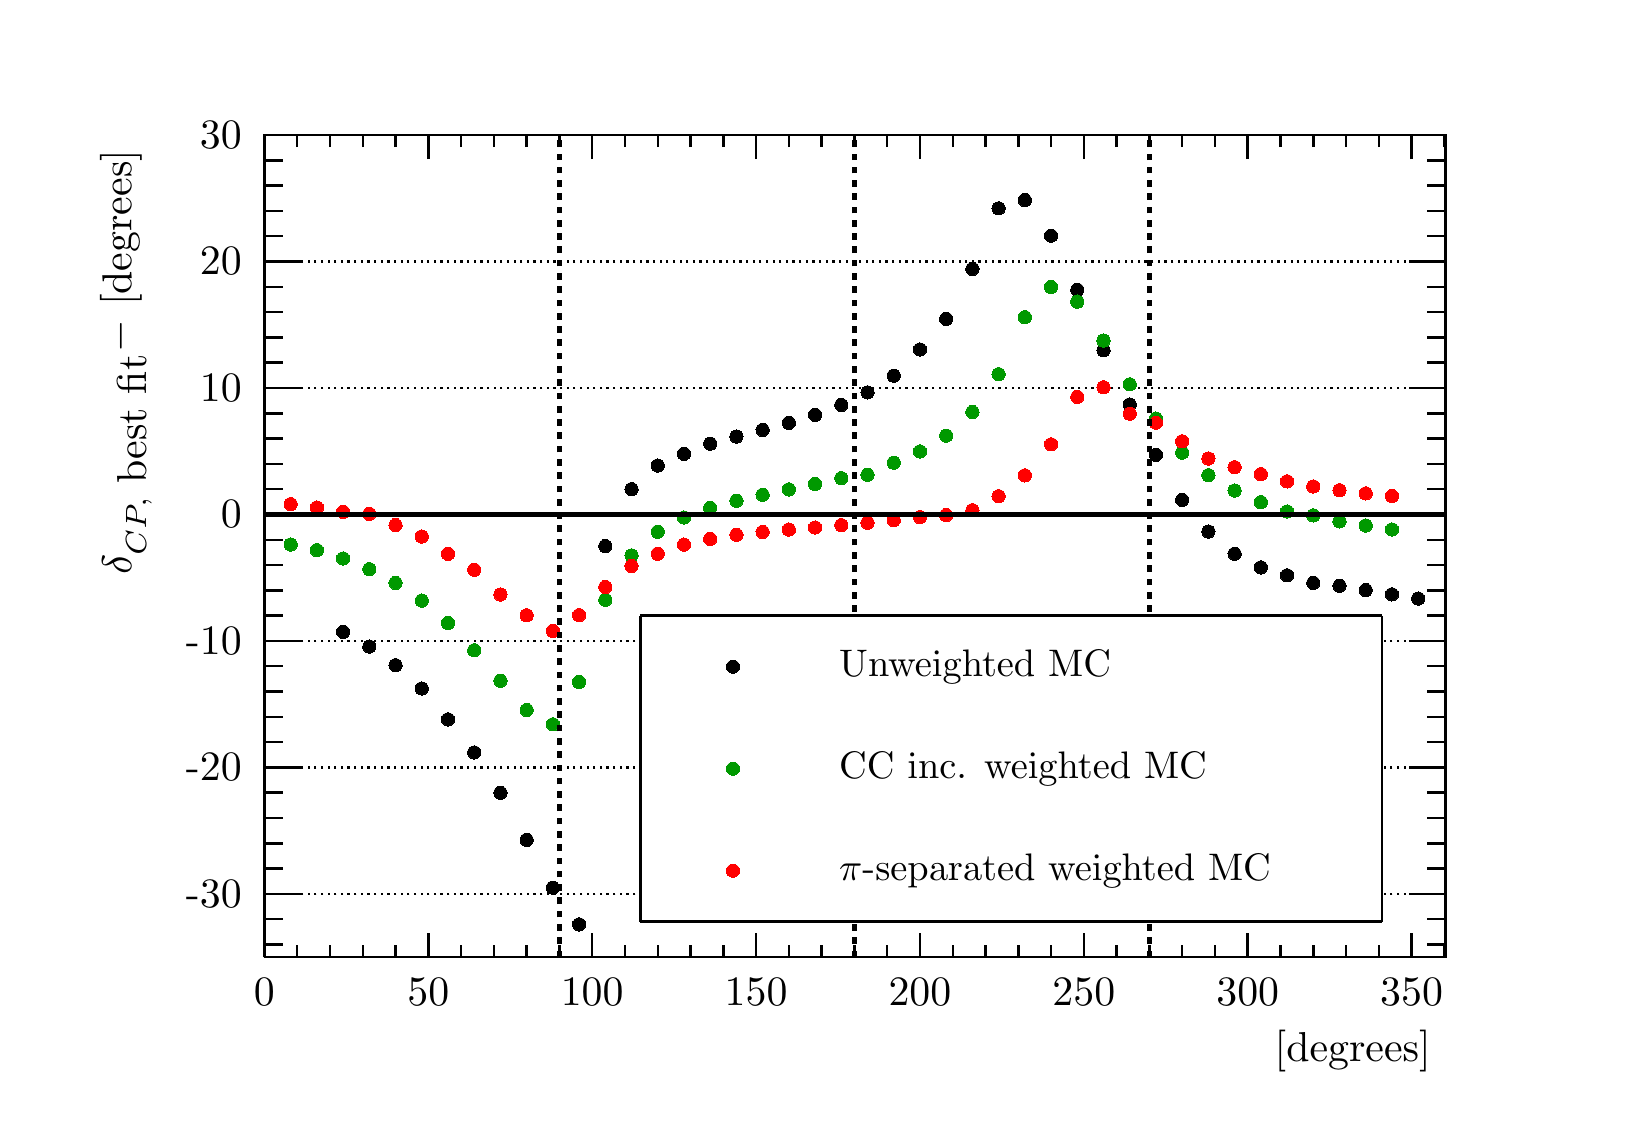
\begin{tikzpicture}
\pgfdeclareplotmark{cross} {
\pgfpathmoveto{\pgfpoint{-0.3\pgfplotmarksize}{\pgfplotmarksize}}
\pgfpathlineto{\pgfpoint{+0.3\pgfplotmarksize}{\pgfplotmarksize}}
\pgfpathlineto{\pgfpoint{+0.3\pgfplotmarksize}{0.3\pgfplotmarksize}}
\pgfpathlineto{\pgfpoint{+1\pgfplotmarksize}{0.3\pgfplotmarksize}}
\pgfpathlineto{\pgfpoint{+1\pgfplotmarksize}{-0.3\pgfplotmarksize}}
\pgfpathlineto{\pgfpoint{+0.3\pgfplotmarksize}{-0.3\pgfplotmarksize}}
\pgfpathlineto{\pgfpoint{+0.3\pgfplotmarksize}{-1.\pgfplotmarksize}}
\pgfpathlineto{\pgfpoint{-0.3\pgfplotmarksize}{-1.\pgfplotmarksize}}
\pgfpathlineto{\pgfpoint{-0.3\pgfplotmarksize}{-0.3\pgfplotmarksize}}
\pgfpathlineto{\pgfpoint{-1.\pgfplotmarksize}{-0.3\pgfplotmarksize}}
\pgfpathlineto{\pgfpoint{-1.\pgfplotmarksize}{0.3\pgfplotmarksize}}
\pgfpathlineto{\pgfpoint{-0.3\pgfplotmarksize}{0.3\pgfplotmarksize}}
\pgfpathclose
\pgfusepathqstroke
}
\pgfdeclareplotmark{cross*} {
\pgfpathmoveto{\pgfpoint{-0.3\pgfplotmarksize}{\pgfplotmarksize}}
\pgfpathlineto{\pgfpoint{+0.3\pgfplotmarksize}{\pgfplotmarksize}}
\pgfpathlineto{\pgfpoint{+0.3\pgfplotmarksize}{0.3\pgfplotmarksize}}
\pgfpathlineto{\pgfpoint{+1\pgfplotmarksize}{0.3\pgfplotmarksize}}
\pgfpathlineto{\pgfpoint{+1\pgfplotmarksize}{-0.3\pgfplotmarksize}}
\pgfpathlineto{\pgfpoint{+0.3\pgfplotmarksize}{-0.3\pgfplotmarksize}}
\pgfpathlineto{\pgfpoint{+0.3\pgfplotmarksize}{-1.\pgfplotmarksize}}
\pgfpathlineto{\pgfpoint{-0.3\pgfplotmarksize}{-1.\pgfplotmarksize}}
\pgfpathlineto{\pgfpoint{-0.3\pgfplotmarksize}{-0.3\pgfplotmarksize}}
\pgfpathlineto{\pgfpoint{-1.\pgfplotmarksize}{-0.3\pgfplotmarksize}}
\pgfpathlineto{\pgfpoint{-1.\pgfplotmarksize}{0.3\pgfplotmarksize}}
\pgfpathlineto{\pgfpoint{-0.3\pgfplotmarksize}{0.3\pgfplotmarksize}}
\pgfpathclose
\pgfusepathqfillstroke
}
\pgfdeclareplotmark{newstar} {
\pgfpathmoveto{\pgfqpoint{0pt}{\pgfplotmarksize}}
\pgfpathlineto{\pgfqpointpolar{44}{0.5\pgfplotmarksize}}
\pgfpathlineto{\pgfqpointpolar{18}{\pgfplotmarksize}}
\pgfpathlineto{\pgfqpointpolar{-20}{0.5\pgfplotmarksize}}
\pgfpathlineto{\pgfqpointpolar{-54}{\pgfplotmarksize}}
\pgfpathlineto{\pgfqpointpolar{-90}{0.5\pgfplotmarksize}}
\pgfpathlineto{\pgfqpointpolar{234}{\pgfplotmarksize}}
\pgfpathlineto{\pgfqpointpolar{198}{0.5\pgfplotmarksize}}
\pgfpathlineto{\pgfqpointpolar{162}{\pgfplotmarksize}}
\pgfpathlineto{\pgfqpointpolar{134}{0.5\pgfplotmarksize}}
\pgfpathclose
\pgfusepathqstroke
}
\pgfdeclareplotmark{newstar*} {
\pgfpathmoveto{\pgfqpoint{0pt}{\pgfplotmarksize}}
\pgfpathlineto{\pgfqpointpolar{44}{0.5\pgfplotmarksize}}
\pgfpathlineto{\pgfqpointpolar{18}{\pgfplotmarksize}}
\pgfpathlineto{\pgfqpointpolar{-20}{0.5\pgfplotmarksize}}
\pgfpathlineto{\pgfqpointpolar{-54}{\pgfplotmarksize}}
\pgfpathlineto{\pgfqpointpolar{-90}{0.5\pgfplotmarksize}}
\pgfpathlineto{\pgfqpointpolar{234}{\pgfplotmarksize}}
\pgfpathlineto{\pgfqpointpolar{198}{0.5\pgfplotmarksize}}
\pgfpathlineto{\pgfqpointpolar{162}{\pgfplotmarksize}}
\pgfpathlineto{\pgfqpointpolar{134}{0.5\pgfplotmarksize}}
\pgfpathclose
\pgfusepathqfillstroke
}
\definecolor{c}{rgb}{1,1,1};
\draw [color=c, fill=c] (0,0) rectangle (20,13.5603);
\draw [color=c, fill=c] (3,1.76284) rectangle (18,12.2043);
\definecolor{c}{rgb}{0,0,0};
\draw [c,line width=0.9] (3,1.76284) -- (3,12.2043) -- (18,12.2043) -- (18,1.76284) -- (3,1.76284);
\definecolor{c}{rgb}{1,1,1};
\draw [color=c, fill=c] (3,1.76284) rectangle (18,12.2043);
\definecolor{c}{rgb}{0,0,0};
\draw [c,line width=0.9] (3,1.76284) -- (3,12.2043) -- (18,12.2043) -- (18,1.76284) -- (3,1.76284);
\draw [c,line width=0.9] (3,1.76284) -- (18,1.76284);
\draw [c,line width=0.9] (3,12.2043) -- (18,12.2043);
\draw [c,line width=0.9] (3,1.76284) -- (3,12.2043);
\draw [c,dash pattern=on 0.80pt off 1.60pt ,line width=0.9] (18,2.56602) -- (3,2.56602);
\draw [c,dash pattern=on 0.80pt off 1.60pt ,line width=0.9] (18,4.17239) -- (3,4.17239);
\draw [c,dash pattern=on 0.80pt off 1.60pt ,line width=0.9] (18,5.77877) -- (3,5.77877);
\draw [c,dash pattern=on 0.80pt off 1.60pt ,line width=0.9] (18,7.38514) -- (3,7.38514);
\draw [c,dash pattern=on 0.80pt off 1.60pt ,line width=0.9] (18,8.99151) -- (3,8.99151);
\draw [c,dash pattern=on 0.80pt off 1.60pt ,line width=0.9] (18,10.5979) -- (3,10.5979);
\draw [c,dash pattern=on 0.80pt off 1.60pt ,line width=0.9] (18,12.2043) -- (3,12.2043);
\draw [c,dash pattern=on 0.80pt off 1.60pt ,line width=0.9] (18,2.56602) -- (3,2.56602);
\draw [c,line width=0.9] (18,1.76284) -- (18,12.2043);
\draw [c,line width=0.9] (3,1.76284) -- (18,1.76284);
\draw [c,line width=0.9] (3,2.06794) -- (3,1.76284);
\draw [c,line width=0.9] (3.41625,1.91539) -- (3.41625,1.76284);
\draw [c,line width=0.9] (3.8325,1.91539) -- (3.8325,1.76284);
\draw [c,line width=0.9] (4.24875,1.91539) -- (4.24875,1.76284);
\draw [c,line width=0.9] (4.665,1.91539) -- (4.665,1.76284);
\draw [c,line width=0.9] (5.08125,2.06794) -- (5.08125,1.76284);
\draw [c,line width=0.9] (5.4975,1.91539) -- (5.4975,1.76284);
\draw [c,line width=0.9] (5.91375,1.91539) -- (5.91375,1.76284);
\draw [c,line width=0.9] (6.33,1.91539) -- (6.33,1.76284);
\draw [c,line width=0.9] (6.74625,1.91539) -- (6.74625,1.76284);
\draw [c,line width=0.9] (7.1625,2.06794) -- (7.1625,1.76284);
\draw [c,line width=0.9] (7.57875,1.91539) -- (7.57875,1.76284);
\draw [c,line width=0.9] (7.99501,1.91539) -- (7.99501,1.76284);
\draw [c,line width=0.9] (8.41126,1.91539) -- (8.41126,1.76284);
\draw [c,line width=0.9] (8.82751,1.91539) -- (8.82751,1.76284);
\draw [c,line width=0.9] (9.24376,2.06794) -- (9.24376,1.76284);
\draw [c,line width=0.9] (9.66001,1.91539) -- (9.66001,1.76284);
\draw [c,line width=0.9] (10.0763,1.91539) -- (10.0763,1.76284);
\draw [c,line width=0.9] (10.4925,1.91539) -- (10.4925,1.76284);
\draw [c,line width=0.9] (10.9088,1.91539) -- (10.9088,1.76284);
\draw [c,line width=0.9] (11.325,2.06794) -- (11.325,1.76284);
\draw [c,line width=0.9] (11.7413,1.91539) -- (11.7413,1.76284);
\draw [c,line width=0.9] (12.1575,1.91539) -- (12.1575,1.76284);
\draw [c,line width=0.9] (12.5738,1.91539) -- (12.5738,1.76284);
\draw [c,line width=0.9] (12.99,1.91539) -- (12.99,1.76284);
\draw [c,line width=0.9] (13.4063,2.06794) -- (13.4063,1.76284);
\draw [c,line width=0.9] (13.8225,1.91539) -- (13.8225,1.76284);
\draw [c,line width=0.9] (14.2388,1.91539) -- (14.2388,1.76284);
\draw [c,line width=0.9] (14.655,1.91539) -- (14.655,1.76284);
\draw [c,line width=0.9] (15.0713,1.91539) -- (15.0713,1.76284);
\draw [c,line width=0.9] (15.4875,2.06794) -- (15.4875,1.76284);
\draw [c,line width=0.9] (15.9038,1.91539) -- (15.9038,1.76284);
\draw [c,line width=0.9] (16.32,1.91539) -- (16.32,1.76284);
\draw [c,line width=0.9] (16.7363,1.91539) -- (16.7363,1.76284);
\draw [c,line width=0.9] (17.1525,1.91539) -- (17.1525,1.76284);
\draw [c,line width=0.9] (17.5688,2.06794) -- (17.5688,1.76284);
\draw [c,line width=0.9] (17.5688,2.06794) -- (17.5688,1.76284);
\draw [c,line width=0.9] (17.985,1.91539) -- (17.985,1.76284);
\draw [anchor=base] (3,1.15262) node[scale=1.51215, color=c, rotate=0]{0};
\draw [anchor=base] (5.08125,1.15262) node[scale=1.51215, color=c, rotate=0]{50};
\draw [anchor=base] (7.1625,1.15262) node[scale=1.51215, color=c, rotate=0]{100};
\draw [anchor=base] (9.24376,1.15262) node[scale=1.51215, color=c, rotate=0]{150};
\draw [anchor=base] (11.325,1.15262) node[scale=1.51215, color=c, rotate=0]{200};
\draw [anchor=base] (13.4063,1.15262) node[scale=1.51215, color=c, rotate=0]{250};
\draw [anchor=base] (15.4875,1.15262) node[scale=1.51215, color=c, rotate=0]{300};
\draw [anchor=base] (17.5688,1.15262) node[scale=1.51215, color=c, rotate=0]{350};
\draw [anchor= east] (18,0.569532) node[scale=1.51215, color=c, rotate=0]{\dcpTrue [degrees]};
\draw [c,line width=0.9] (3,12.2043) -- (18,12.2043);
\draw [c,line width=0.9] (3,11.8991) -- (3,12.2043);
\draw [c,line width=0.9] (3.41625,12.0517) -- (3.41625,12.2043);
\draw [c,line width=0.9] (3.8325,12.0517) -- (3.8325,12.2043);
\draw [c,line width=0.9] (4.24875,12.0517) -- (4.24875,12.2043);
\draw [c,line width=0.9] (4.665,12.0517) -- (4.665,12.2043);
\draw [c,line width=0.9] (5.08125,11.8991) -- (5.08125,12.2043);
\draw [c,line width=0.9] (5.4975,12.0517) -- (5.4975,12.2043);
\draw [c,line width=0.9] (5.91375,12.0517) -- (5.91375,12.2043);
\draw [c,line width=0.9] (6.33,12.0517) -- (6.33,12.2043);
\draw [c,line width=0.9] (6.74625,12.0517) -- (6.74625,12.2043);
\draw [c,line width=0.9] (7.1625,11.8991) -- (7.1625,12.2043);
\draw [c,line width=0.9] (7.57875,12.0517) -- (7.57875,12.2043);
\draw [c,line width=0.9] (7.99501,12.0517) -- (7.99501,12.2043);
\draw [c,line width=0.9] (8.41126,12.0517) -- (8.41126,12.2043);
\draw [c,line width=0.9] (8.82751,12.0517) -- (8.82751,12.2043);
\draw [c,line width=0.9] (9.24376,11.8991) -- (9.24376,12.2043);
\draw [c,line width=0.9] (9.66001,12.0517) -- (9.66001,12.2043);
\draw [c,line width=0.9] (10.0763,12.0517) -- (10.0763,12.2043);
\draw [c,line width=0.9] (10.4925,12.0517) -- (10.4925,12.2043);
\draw [c,line width=0.9] (10.9088,12.0517) -- (10.9088,12.2043);
\draw [c,line width=0.9] (11.325,11.8991) -- (11.325,12.2043);
\draw [c,line width=0.9] (11.7413,12.0517) -- (11.7413,12.2043);
\draw [c,line width=0.9] (12.1575,12.0517) -- (12.1575,12.2043);
\draw [c,line width=0.9] (12.5738,12.0517) -- (12.5738,12.2043);
\draw [c,line width=0.9] (12.99,12.0517) -- (12.99,12.2043);
\draw [c,line width=0.9] (13.4063,11.8991) -- (13.4063,12.2043);
\draw [c,line width=0.9] (13.8225,12.0517) -- (13.8225,12.2043);
\draw [c,line width=0.9] (14.2388,12.0517) -- (14.2388,12.2043);
\draw [c,line width=0.9] (14.655,12.0517) -- (14.655,12.2043);
\draw [c,line width=0.9] (15.0713,12.0517) -- (15.0713,12.2043);
\draw [c,line width=0.9] (15.4875,11.8991) -- (15.4875,12.2043);
\draw [c,line width=0.9] (15.9038,12.0517) -- (15.9038,12.2043);
\draw [c,line width=0.9] (16.32,12.0517) -- (16.32,12.2043);
\draw [c,line width=0.9] (16.7363,12.0517) -- (16.7363,12.2043);
\draw [c,line width=0.9] (17.1525,12.0517) -- (17.1525,12.2043);
\draw [c,line width=0.9] (17.5688,11.8991) -- (17.5688,12.2043);
\draw [c,line width=0.9] (17.5688,11.8991) -- (17.5688,12.2043);
\draw [c,line width=0.9] (17.985,12.0517) -- (17.985,12.2043);
\draw [c,line width=0.9] (3,1.76284) -- (3,12.2043);
\draw [c,line width=0.9] (3.462,2.56602) -- (3,2.56602);
\draw [c,line width=0.9] (3.231,2.8873) -- (3,2.8873);
\draw [c,line width=0.9] (3.231,3.20857) -- (3,3.20857);
\draw [c,line width=0.9] (3.231,3.52985) -- (3,3.52985);
\draw [c,line width=0.9] (3.231,3.85112) -- (3,3.85112);
\draw [c,line width=0.9] (3.462,4.17239) -- (3,4.17239);
\draw [c,line width=0.9] (3.231,4.49367) -- (3,4.49367);
\draw [c,line width=0.9] (3.231,4.81494) -- (3,4.81494);
\draw [c,line width=0.9] (3.231,5.13622) -- (3,5.13622);
\draw [c,line width=0.9] (3.231,5.45749) -- (3,5.45749);
\draw [c,line width=0.9] (3.462,5.77877) -- (3,5.77877);
\draw [c,line width=0.9] (3.231,6.10004) -- (3,6.10004);
\draw [c,line width=0.9] (3.231,6.42132) -- (3,6.42132);
\draw [c,line width=0.9] (3.231,6.74259) -- (3,6.74259);
\draw [c,line width=0.9] (3.231,7.06386) -- (3,7.06386);
\draw [c,line width=0.9] (3.462,7.38514) -- (3,7.38514);
\draw [c,line width=0.9] (3.231,7.70641) -- (3,7.70641);
\draw [c,line width=0.9] (3.231,8.02769) -- (3,8.02769);
\draw [c,line width=0.9] (3.231,8.34896) -- (3,8.34896);
\draw [c,line width=0.9] (3.231,8.67024) -- (3,8.67024);
\draw [c,line width=0.9] (3.462,8.99151) -- (3,8.99151);
\draw [c,line width=0.9] (3.231,9.31279) -- (3,9.31279);
\draw [c,line width=0.9] (3.231,9.63406) -- (3,9.63406);
\draw [c,line width=0.9] (3.231,9.95533) -- (3,9.95533);
\draw [c,line width=0.9] (3.231,10.2766) -- (3,10.2766);
\draw [c,line width=0.9] (3.462,10.5979) -- (3,10.5979);
\draw [c,line width=0.9] (3.231,10.9192) -- (3,10.9192);
\draw [c,line width=0.9] (3.231,11.2404) -- (3,11.2404);
\draw [c,line width=0.9] (3.231,11.5617) -- (3,11.5617);
\draw [c,line width=0.9] (3.231,11.883) -- (3,11.883);
\draw [c,line width=0.9] (3.462,12.2043) -- (3,12.2043);
\draw [c,line width=0.9] (3.462,2.56602) -- (3,2.56602);
\draw [c,line width=0.9] (3.231,2.24475) -- (3,2.24475);
\draw [c,line width=0.9] (3.231,1.92347) -- (3,1.92347);
\draw [anchor= east] (2.9,2.56602) node[scale=1.51215, color=c, rotate=0]{-30};
\draw [anchor= east] (2.9,4.17239) node[scale=1.51215, color=c, rotate=0]{-20};
\draw [anchor= east] (2.9,5.77877) node[scale=1.51215, color=c, rotate=0]{-10};
\draw [anchor= east] (2.9,7.38514) node[scale=1.51215, color=c, rotate=0]{0};
\draw [anchor= east] (2.9,8.99151) node[scale=1.51215, color=c, rotate=0]{10};
\draw [anchor= east] (2.9,10.5979) node[scale=1.51215, color=c, rotate=0]{20};
\draw [anchor= east] (2.9,12.2043) node[scale=1.51215, color=c, rotate=0]{30};
\draw [anchor= east] (1.24,12.2043) node[scale=1.51215, color=c, rotate=90]{$\delta_{CP,~\textrm{best fit}} - \dcpTrue$ [degrees]};
\draw [c,line width=0.9] (18,1.76284) -- (18,12.2043);
\draw [c,line width=0.9] (17.538,2.56602) -- (18,2.56602);
\draw [c,line width=0.9] (17.769,2.8873) -- (18,2.8873);
\draw [c,line width=0.9] (17.769,3.20857) -- (18,3.20857);
\draw [c,line width=0.9] (17.769,3.52985) -- (18,3.52985);
\draw [c,line width=0.9] (17.769,3.85112) -- (18,3.85112);
\draw [c,line width=0.9] (17.538,4.17239) -- (18,4.17239);
\draw [c,line width=0.9] (17.769,4.49367) -- (18,4.49367);
\draw [c,line width=0.9] (17.769,4.81494) -- (18,4.81494);
\draw [c,line width=0.9] (17.769,5.13622) -- (18,5.13622);
\draw [c,line width=0.9] (17.769,5.45749) -- (18,5.45749);
\draw [c,line width=0.9] (17.538,5.77877) -- (18,5.77877);
\draw [c,line width=0.9] (17.769,6.10004) -- (18,6.10004);
\draw [c,line width=0.9] (17.769,6.42132) -- (18,6.42132);
\draw [c,line width=0.9] (17.769,6.74259) -- (18,6.74259);
\draw [c,line width=0.9] (17.769,7.06386) -- (18,7.06386);
\draw [c,line width=0.9] (17.538,7.38514) -- (18,7.38514);
\draw [c,line width=0.9] (17.769,7.70641) -- (18,7.70641);
\draw [c,line width=0.9] (17.769,8.02769) -- (18,8.02769);
\draw [c,line width=0.9] (17.769,8.34896) -- (18,8.34896);
\draw [c,line width=0.9] (17.769,8.67024) -- (18,8.67024);
\draw [c,line width=0.9] (17.538,8.99151) -- (18,8.99151);
\draw [c,line width=0.9] (17.769,9.31279) -- (18,9.31279);
\draw [c,line width=0.9] (17.769,9.63406) -- (18,9.63406);
\draw [c,line width=0.9] (17.769,9.95533) -- (18,9.95533);
\draw [c,line width=0.9] (17.769,10.2766) -- (18,10.2766);
\draw [c,line width=0.9] (17.538,10.5979) -- (18,10.5979);
\draw [c,line width=0.9] (17.769,10.9192) -- (18,10.9192);
\draw [c,line width=0.9] (17.769,11.2404) -- (18,11.2404);
\draw [c,line width=0.9] (17.769,11.5617) -- (18,11.5617);
\draw [c,line width=0.9] (17.769,11.883) -- (18,11.883);
\draw [c,line width=0.9] (17.538,12.2043) -- (18,12.2043);
\draw [c,line width=0.9] (17.538,2.56602) -- (18,2.56602);
\draw [c,line width=0.9] (17.769,2.24475) -- (18,2.24475);
\draw [c,line width=0.9] (17.769,1.92347) -- (18,1.92347);
\foreach \P in {(3.999,5.89376), (4.332,5.70739), (4.665,5.4712), (4.998,5.1748), (5.331,4.78284), (5.664,4.36308), (5.997,3.8498), (6.33,3.25239), (6.663,2.64556), (6.996,2.17921), (7.329,6.98376), (7.662,7.70655), (7.99501,8.00579),
 (8.32801,8.15546), (8.66101,8.28375), (8.99401,8.37416), (9.32701,8.4587), (9.66001,8.54915), (9.99301,8.6505), (10.326,8.77565), (10.659,8.93528), (10.992,9.14738), (11.325,9.48058), (11.658,9.86968), (11.991,10.5031), (12.324,11.2726),
 (12.657,11.3777), (12.99,10.925), (13.323,10.2384), (13.656,9.4696), (13.989,8.78134), (14.322,8.14301), (14.655,7.56952), (14.988,7.1674), (15.321,6.88575), (15.654,6.71275), (15.987,6.6118), (16.32,6.5165), (16.653,6.47938), (16.986,6.42435),
 (17.319,6.3704), (17.652,6.3169)}{\draw[mark options={color=c,fill=c},mark size=2.402402pt, line width=0.000000pt, mark=*] plot coordinates {\P};}
\definecolor{c}{rgb}{1,1,1};
\draw [color=c, fill=c] (2,12.7467) rectangle (18,13.4925);
\definecolor{c}{rgb}{0,0,0};
%\draw (10,13.1196) node[scale=1.38614, color=c, rotate=0]{Unweighted MC};
\definecolor{c}{rgb}{0,0.6,0};
\foreach \P in {(3.333,7.00321), (3.666,6.93165), (3.999,6.82615), (4.332,6.69018), (4.665,6.5158), (4.998,6.29084), (5.331,6.00512), (5.664,5.66082), (5.997,5.27369), (6.33,4.90165), (6.663,4.72004), (6.996,5.25847), (7.329,6.30145),
 (7.662,6.86524), (7.99501,7.16582), (8.32801,7.34643), (8.66101,7.46856), (8.99401,7.55965), (9.32701,7.63485), (9.66001,7.70337), (9.99301,7.7716), (10.326,7.8461), (10.659,7.8886), (10.992,8.04253), (11.325,8.18552), (11.658,8.38589),
 (11.991,8.68617), (12.324,9.16637), (12.657,9.89039), (12.99,10.2729), (13.323,10.0878), (13.656,9.5933), (13.989,9.03807), (14.322,8.60232), (14.655,8.17044), (14.988,7.88401), (15.321,7.68859), (15.654,7.54124), (15.987,7.42269), (16.32,7.37364),
 (16.653,7.29735), (16.986,7.24452), (17.319,7.19439)}{\draw[mark options={color=c,fill=c},mark size=2.402402pt, line width=0.000000pt, mark=*] plot coordinates {\P};}
\definecolor{c}{rgb}{1,0,0};
\foreach \P in {(3.333,7.51624), (3.666,7.47326), (3.999,7.41876), (4.332,7.39304), (4.665,7.25022), (4.998,7.1046), (5.331,6.88581), (5.664,6.68283), (5.997,6.36882), (6.33,6.10472), (6.663,5.90619), (6.996,6.10632), (7.329,6.46369),
 (7.662,6.73066), (7.99501,6.88634), (8.32801,7.0018), (8.66101,7.07409), (8.99401,7.12634), (9.32701,7.16291), (9.66001,7.19333), (9.99301,7.2192), (10.326,7.24928), (10.659,7.27962), (10.992,7.31358), (11.325,7.351), (11.658,7.37707),
 (11.991,7.43904), (12.324,7.61704), (12.657,7.88169), (12.99,8.27566), (13.323,8.87789), (13.656,9.00015), (13.989,8.66472), (14.322,8.54999), (14.655,8.3143), (14.988,8.09578), (15.321,7.9855), (15.654,7.89718), (15.987,7.80543), (16.32,7.74059),
 (16.653,7.69268), (16.986,7.65291), (17.319,7.61818)}{\draw[mark options={color=c,fill=c},mark size=2.402402pt, line width=0.000000pt, mark=*] plot coordinates {\P};}
\definecolor{c}{rgb}{0,0,0};
\draw [c,line width=1.8] (3,7.38514) -- (17.985,7.38514);
\draw [c,dash pattern=on 2.40pt off 2.40pt ,line width=1.8] (6.74625,1.76284) -- (6.74625,12.2043);
\draw [c,dash pattern=on 2.40pt off 2.40pt ,line width=1.8] (10.4925,1.76284) -- (10.4925,12.2043);
\draw [c,dash pattern=on 2.40pt off 2.40pt ,line width=1.8] (14.2388,1.76284) -- (14.2388,12.2043);
\definecolor{c}{rgb}{1,1,1};
\draw [color=c, fill=c] (7.77305,2.21277) rectangle (17.1915,6.09929);
\definecolor{c}{rgb}{0,0,0};
\draw [c,line width=0.9] (7.77305,2.21277) -- (17.1915,2.21277);
\draw [c,line width=0.9] (17.1915,2.21277) -- (17.1915,6.09929);
\draw [c,line width=0.9] (17.1915,6.09929) -- (7.77305,6.09929);
\draw [c,line width=0.9] (7.77305,6.09929) -- (7.77305,2.21277);
\draw [anchor= west] (10.1277,5.45154) node[scale=1.38614, color=c, rotate=0]{Unweighted MC};
\foreach \P in {(8.95035,5.45154)}{\draw[mark options={color=c,fill=c},mark size=2.402402pt, line width=0.000000pt, mark=*] plot coordinates {\P};}
\draw [anchor= west] (10.1277,4.15603) node[scale=1.38614, color=c, rotate=0]{CC inc. weighted MC};
\definecolor{c}{rgb}{0,0.6,0};
\foreach \P in {(8.95035,4.15603)}{\draw[mark options={color=c,fill=c},mark size=2.402402pt, line width=0.000000pt, mark=*] plot coordinates {\P};}
\definecolor{c}{rgb}{0,0,0};
\draw [anchor= west] (10.1277,2.86052) node[scale=1.38614, color=c, rotate=0]{$\pi$-separated weighted MC};
\definecolor{c}{rgb}{1,0,0};
\foreach \P in {(8.95035,2.86052)}{\draw[mark options={color=c,fill=c},mark size=2.402402pt, line width=0.000000pt, mark=*] plot coordinates {\P};}
\end{tikzpicture}
